\subsection{Homomorphic Logic Aggregation}\label{block: minmax}
Most existing homomorphically encrypted database techniques~\cite{aphadb, heda} 
only support arithmetic aggregation (e.g., $\dbsum$ or $\dbavg$).
To support logic aggregation 
such as $\dbmin$, $\dbmax$, $\dbtopk$ and SQL statement such as $\orderby$, 
%we first propose a new set of two-input homomorphic operators to carry out
%$\dbmin$ and $\dbmax$ between two ciphertexts. Next, we propose an aggregation
we propose new two-input logic operators
that can be used to construct arbitrary logic aggregation functions. 
Due to space limitation, we use $\hommin$ as an example in this section. 
Our methodology applies generally to other types of logic aggregations.
% homomorphic $\dbmin$ operator $\hommin$
% and construct logic aggregation 
% $\homminagg$.


\begin{algorithm}[t!]
    % \tiny
    \caption{$\hommin$}
    \label{algo: hommin}
    \SetKwInOut{Input}{Input}\SetKwInOut{Output}{Output}\SetKwInOut{Return}{Return}
    \Input{Two LWE ciphertexts $ct_a = \lwe(a), ct_b = \lwe(b)$.}
    \Input{A bootstrapping key $\bBK$.}
    \Output{A LWE ciphertext $ct_{O} = \lwe(\dbmin(a,b))$.}
    $ct \leftarrow \homcomp(ct_a, ct_b, \leq)$ \\
    $C \leftarrow \cb(ct,\bBK)$ \\
    $ct_O \leftarrow \cmux(C, ct_a, ct_b)$ \\
    
    \Return{$ct_{O} = \lwe(\dbmin(a,b))$}
\end{algorithm}

\begin{algorithm}[t!]
    % \tiny
    \caption{$\homminagg$}
    \label{algo: homminagg}
    \SetKwInOut{Input}{Input}\SetKwInOut{Output}{Output}\SetKwInOut{Return}{Return}
    \Input{An RLWE ciphertext of the aggregated column $ct = \rlwe(\Tilde{m})$ where
    $\Tilde{m}_i = m_i$ for $i \in \mathbb{Z}_{\dbtabrowsize}$.}
    \Input{Filtered result $cf=
    (cf_{0}, cf_{1}, ... ,cf_{\dbtabrowsize - 1})$, where
    $cf_i = \lwe(f_i)$, $f_i = 0$ or $1$.}
    \Input{The pre-defined constant $\lwenan$.}
    \Input{A bootstrapping key $\bBK$.}
    \Output{A LWE ciphertext $ct_{O} = \lwe(\dbmin(m_{t_0}, ...,m_{t_{f-1}}))$ where
    $f =  {\textstyle \sum_{i=0}^{\dbtabrowsize - 1}}f_i$
    and $f_{t_0}, f_{t_1}, ..., f_{t_{f-1}} = 1$.}
    $\mathbf{ct} \leftarrow \sei(ct) = (ct_0, ct_1, ...,ct_{\dbtabrowsize-1})$ \\
    \For{$i = 0$ \KwTo $\dbtabrowsize - 1$}
    {
        $C_i \leftarrow \cb(cf_i, \bBK)$ \\
        $ct_i \leftarrow \cmux(C,ct_i,\lwenan)$ \\
    }
    \For{$i = 0$ \KwTo $\log_{2}{\dbtabrowsize} - 1$}
    {
        \For{$j = 0$ \KwTo $2^{\log_{2}{\dbtabrowsize} - i - 1} - 1$}
        {
            $ct_{2^{i+1}\cdot j} \leftarrow 
            \hommin(ct_{2^{i+1} \cdot j}, ct_{2^{i+1} \cdot j + 2^{i}}, \bBK)$ \\
        }
    }
    \Return{$ct_{O} = ct_{}0$}
\end{algorithm}

\subsubsection{Homomorphic $\dbmin$ and $\dbmin$ aggregation}
While there exists prior works~\cite{ckkscomparison, pegasus} 
for computing $\hommin$ and $\hommax$ operators, 
such techniques cannot be directly applied to a homomorphically encrypted database
due to two major obstacles.
The first obstacle is the low evaluation speed and unstable aggregation precision.
For example, while~\cite{ckkscomparison} can achieve high-precision $\hommin$ evaluation,
the method incurs a large number of latency overheads. On the other hand,
although~\cite{pegasus} can evaluate $\hommin$ and $\hommax$ relatively fast 
(but still slower than our proposed technique),
the technique suffers from the low precision ($<$ 6-bit) problem.
The second obstacle is how to evaluate logic aggregations
only on filtered rows. For a set of homomorphically filtered
results, the server cannot distinguish between an attribute value originally encrypted
to be zero and a filtered attribute that is set to be zero. Therefore, when performing
operations such as $\hommin$, we can produce incorrect results if we aggregate on invalid rows
that are marked as zeroes because they are filtered by the SQL statements.
% In a homomorphically encrypted database, 
% the number of selected records  
% and the values of selected records 
% are protected throughout the whole process.
% For instance, we could not distinguish the ciphertext of selected entries 
% between all entry ciphertexts
% $(ct_1, ct_2, ...,ct_{\abs{\mathcal{T}}_r})$.
% Therefore, it is hard to perform logic operators only on 
% the ciphertexts of selected entries.

To tackle the above two obstacles, we propose a new homomorphic logic aggregation procedure.
To overcome the first barrier, we introduce a new mechanism
to homomorphically evaluate $\dbmin$ (and $\dbmax$). We point out
that, for two numbers $a$ and $b$, prior works~\cite{ckkscomparison, pegasus} adopts the following formula
to compute the $\dbmin$ function.
\begin{equation}
    \dbmin(a, b) = (a \leq b)\text{ } ? \text{ }a\text{ } :\text{ } b
        % \begin{cases}
        %         a, a < b \\
        %         b, a \geq b
        % \end{cases}
    =
    \frac{a+b}{2} - \frac{\abs{a-b}}{2} 
    % \quad \reg{and} \quad
    % \texttt{MAX}(a, b) = \frac{a+b}{2} + \frac{\abs{a-b}}{2}
    \label{formula: sminmax}
\end{equation} 
However, evaluating the absolute function in HE will either be too slow
or too inaccurate. To avoid the absolute function, we propose to implement $\dbmin$ 
using the homomorphic comparison $\homcomp$ proposed in \cref{block: comparison}
and the homomorphic selector $\cmux$  defined in \cref{pre:he_circuits}. Essentially,
we compute
\begin{align}\label{eq:mincmux}
\hommin(a, b) = \gsw(a \leq b)\text{ }?\text{ }ct_a\text{ }:\text{ }ct_b,
\end{align}
where $\gsw(a\leq b)=\cb(\homcomp(ct_a, ct_b, \leq)$. Observe that Eq.~\eqref{eq:mincmux} is precisely Eq.~\eqref{eq:cmux},
and we sketch the full algorithm in \cref{algo: hommin}. That is, using $\homcomp$, 
$a\leq b$ can be homomorphically evaluated with high precision and high evaluation speed.
In addition, since $\cmux$ is also a fast operator (around $1000\times$ faster than
$\homcomp$), our $\hommin$ operator can be both faster and more accurate
than existing solutions~\cite{pegasus,ckkscomparison}.

% We exploit a simple fact that the conditional expressions
% of the initial $\dbmin$ definition could be converted 
% to the MSB value, which could be considered to control signal
% in a homomorphic selector.

% \begin{equation}
%     \begin{aligned}
%         \dbmin(a,b) = 
%             \begin{cases}
%                 a, a < b \\
%                 b, a \geq b
%             \end{cases}
%          = 
%             \begin{cases}
%                 a, \msb(a-b)=1 \\
%                 b, \msb(a-b)=0
%             \end{cases}
%         % \\
%         % \texttt{MAX}(a,b) = 
%         %     \begin{cases}
%         %         a, a \geq b \\
%         %         b, a < b
%         %     \end{cases}
%         % = 
%         %     \begin{cases}
%         %         a, MSB(a-b)=0 \\
%         %         b, MSB(a-b)=1
%         %     \end{cases}
%     \end{aligned}
%     \label{formula: minmax}
% \end{equation}

% \begin{equation}
%     \begin{aligned}
%         \hommin(ct_a, ct_b) = \texttt{CMUX}(CMSB, ct_a, ct_b) 
%         \\
%         \texttt{HomMAX}(ct_a, ct_b) = \texttt{CMUX}(CMSB, ct_b, ct_a)
%     \end{aligned}
%     \label{formula: homminmax}
% \end{equation}

% Here $CMSB$ is the RGSW ciphertext of $\texttt{MSB}(a-b)$.

Next, we solve the second obstacle by defining a constant ciphertext $\lwenan$
encrypting NaN, i.e., a `not a number' ciphertext. As detailed in
\cref{algo: homminagg}, the key idea is simple:
before comparing two LWE ciphertexts, 
we first use the encrypted filtered result $\gsw(\frakt)$
to pre-filter the input ciphertext $ct_i$ by computing 
\begin{align}\label{eq:lwenan}
\gsw(\frakt)\text{ }?\text{ }ct_i\text{ }:\text{ }\lwenan,
\end{align}
which is again a $\cmux$ operation. Note that,
in practice, $\lwenan$ can be initialized to be the largest 
value in the range of the plaintext message space (and the smallest
value in the case of $\hommaxagg$).
% before the $\dbmin$ computation.
% Thus the unsatisfactory rows will be replaced by the 
% gigantic ciphertexts and do not 
% affect the aggregation on satisfying rows.
Then, we can proceed to build a conventional 
min-tree of depth $\log_{2}{\dbtabrowsize}$
to calculate the minimum value over all rows in the attribute
column. 
The complexity analysis of the algorithm is provided in 
\cref{lemma: homminagg} (the proof can be found in the Appendix).

\begin{lemma}
    In \cref{algo: homminagg}
    the number of homomorphic \cmux gates is 
    $2\dbtabrowsize - 1$. 
    The number of homomorphic 
    $\cb$ operators is 
    $2\dbtabrowsize -1$,
    and the number of homomorphic 
    $\homcomp$ operators is
    $\dbtabrowsize -1$.
    \label{lemma: homminagg}
\end{lemma}

% \begin{figure}[t!]
%    \begin{center}
%    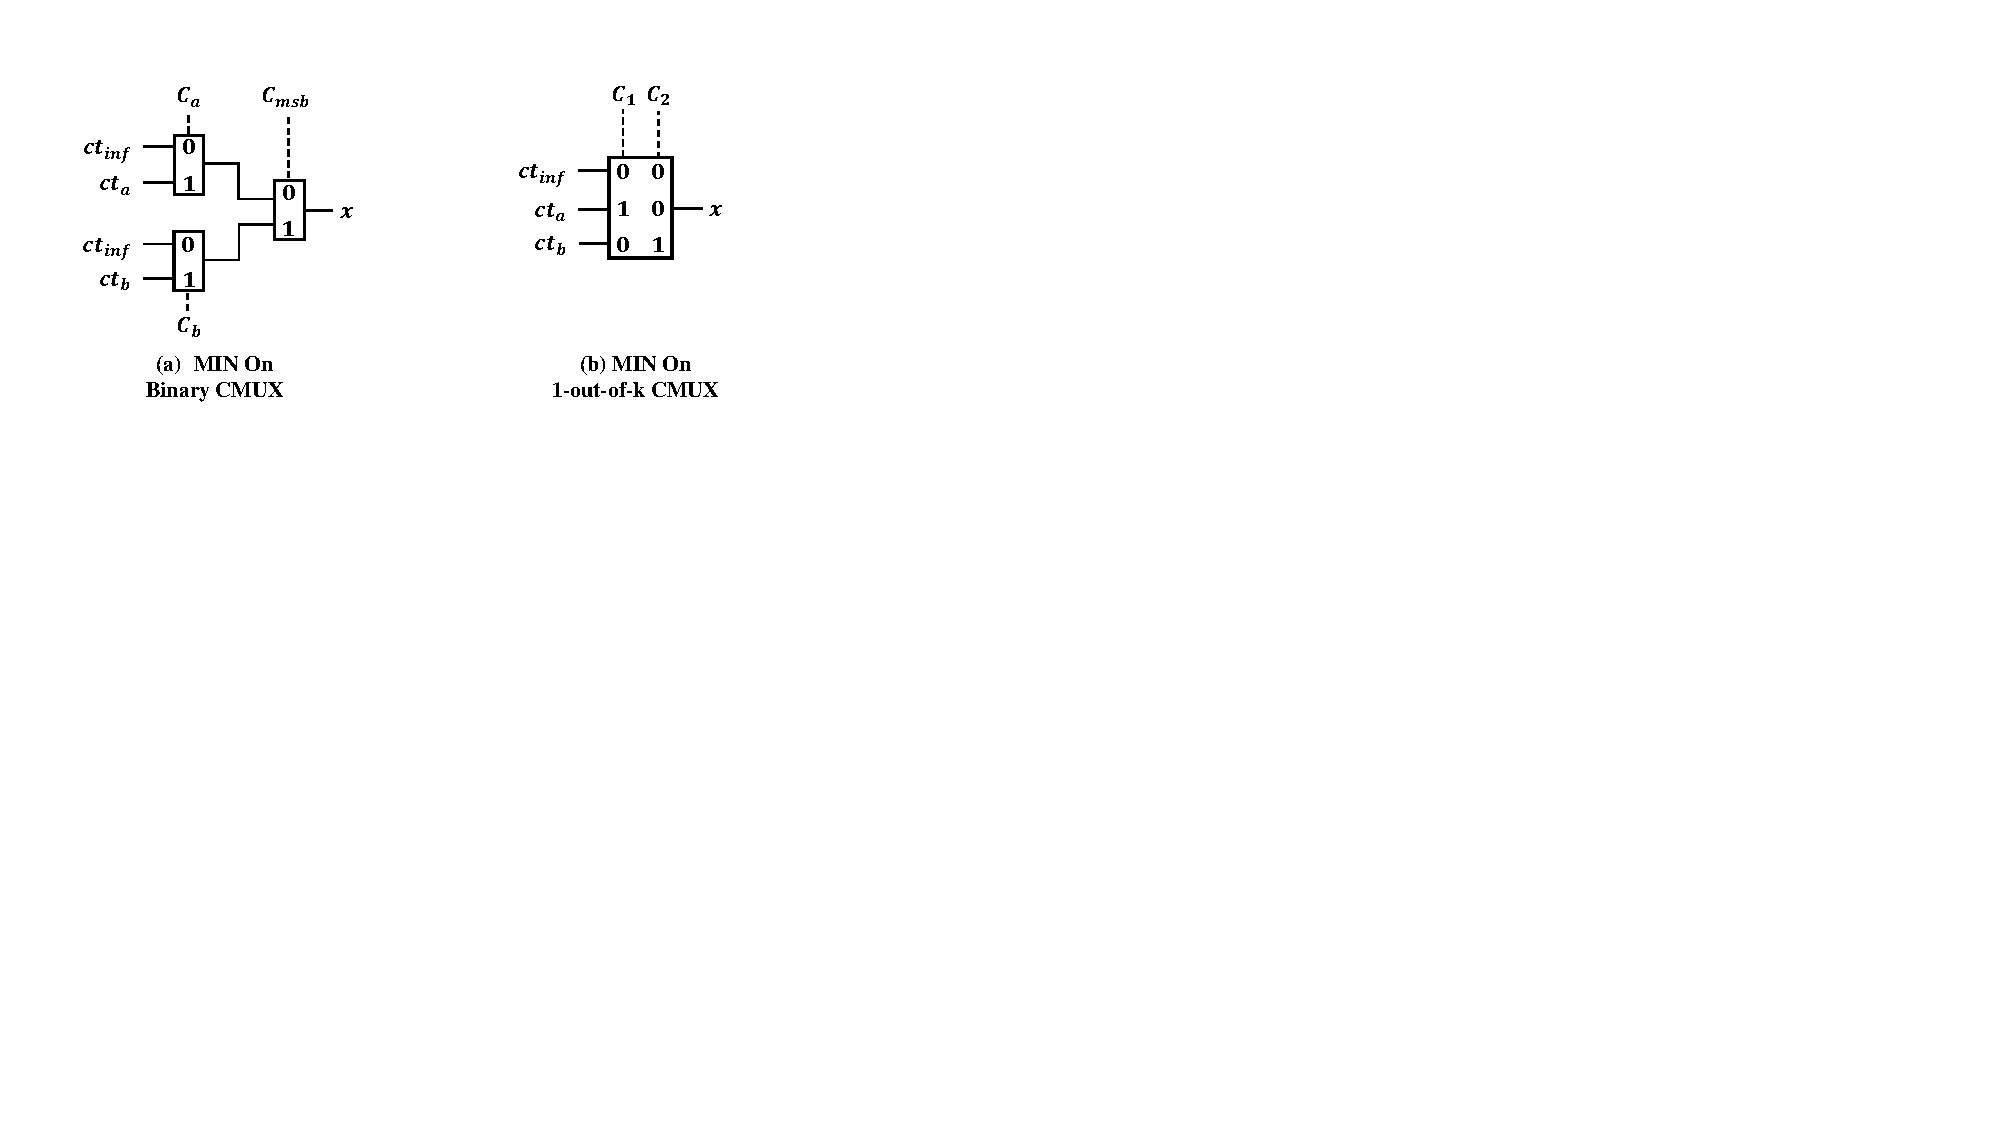
\includegraphics[width=\linewidth]{figure/mincmux.pdf}
%    \end{center}
%     \vspace{-0.5em}
%       \caption{A illustration of $\dbmin$ function on binary $\cmux$ and $\kcmux$.} 
%    \label{fig: mincmux}
%    \vspace{-0.5em}
% \end{figure}

% \begin{algorithm}[t!]
%     % \footnotesize
%     \caption{\texttt{1-out-of-k-CMUX}}
%     \label{algo: kcmux}
%     \SetKwInOut{Input}{Input}\SetKwInOut{Output}{Output}\SetKwInOut{Return}{Return}
%     \Input{$k$ $(\ge 2)$ LWE ciphertexts
%     $ct_0, ct_1, ...,ct_{k-1}$.}
%     \Input{$k-1$ control signals $C_1, C_2, ..., C_{k-1}$ where $C_t = 
%     \rgsw(1)$ and else are $\rgsw(0)$}
%     \Output{An LWE ciphertext $ct_{O} = ct_t$}
%     Initialize $ACC \leftarrow ct_0$. \\
%     \For{$i = 1$ \KwTo $k - 1$}
%     {
%         $temp_i \leftarrow ct_i - ct_0$ \\
%         $ACC \leftarrow ACC + temp_i \odot C_i$
%     }
%     \Return{$ACC$}
% \end{algorithm}

% \subsubsection{Optimizing of $\homminagg$}
% As shown in \cref{fig: mincmux} (a), we depict the \cref{algo: homminagg}
% in the case of two ciphertexts.
% Here, the $C_a$ and $C_b$ are 
% RGSW ciphertexts of the filtered result.
% They first control if $ct_a$ and $ct_b$ will be selected 
% in the latter $\hommin$ function. 
% The result $x_a$ is formulated as 
% \begin{equation}
%     x_a = \texttt{CMUX}(\texttt{CMUX}(ct_{max}, ct_a, C_a),
%     \texttt{CMUX}(ct_{max}, ct_b, C_b), C_{msb})
%     \label{formula: x_a}
% \end{equation}
% 
% However, as the homomorphic predicate evaluation result 
% is a set of LWE ciphertexts, we need to perform
% $\cb$ ciphertext conversion (also known
% as circuit bootstrapping~\cite{DBLP:journals/joc/ChillottiGGI20}) 
% in the first step (line 3-5).
% This takes most of the time in $\homminagg$ (nearly 90\%).
% To reduce the latency, we propose our optimized 
% $\kcmux$ in \cref{algo: kcmux}
% and merge the three $\cmux$
% with three control signals ($C_a, C_b,$ and $C_{msb}$)
% in \cref{fig: mincmux} (a) into one \texttt{1-out-of-3-CMUX}
% with control signals ($C_1$ and $C_2$) shown in \cref{fig: mincmux} (b).
% Here, the result $x_b$ is formulated as 
% \begin{equation}
%     x_b = \texttt{1-out-of-3-CMUX}(ct_{max}, ct_a, ct_b, C_1, C_2)
%     \label{formula: x_b}
% \end{equation}
% 
% The $C_1$ and $C_2$ are the 
% logical combination of $C_a, C_b,$ and $C_{msb}$.
% Therefore, we only need to perform two $\cb$ operators,
% which will reduce the latency
% by about $20\%$.
% Due to space constraints, we detail the exact optimization 
% of $\homminagg$
% in \cref{algo: ophomminagg} and provide
% complexity analysis with proof in \cref{lemma: ophomminagg}.

\subsubsection{Extending to Other Types of Aggregations}
As mentioned, the $\hommax$ and $\hommaxagg$ 
can be implemented in a very similar way as $\hommin$ and $\homminagg$,
except that $\lwenan$ needs to be defined as the smallest value
possible here.
% The \texttt{MIN/MAX-Index} could be constructed by
% changing the input $ct$ of the \cref{algo: homminagg} by the ciphertexts
% encrypts the index of records, \revise{we detail the exact algorithm in ...}.
Meanwhile, to achieve homomorphic $\orderby$, we propose a simple
swap function based on the $\hommin/\hommax$ operators as
% the key part of the sorting function is the swap between ciphertexts
% (including ascending swap and descending swap),
% which is
% We construct other
% operators like (\texttt{MIN/MAX-Index}, \texttt{Top-k}) and sorting
% based on our \texttt{HomMIN/MAX}
\begin{align}
    &\texttt{HASwap}(ct_a,ct_b) =  \hommax(ct_a, ct_b),
    \hommin(ct_a, ct_b)&
    \\
    &\texttt{HDSwap}(ct_a,ct_b) = \hommin(ct_a, ct_b),
    \hommax(ct_a, ct_b),&
\end{align}
depending the ascending ($\texttt{HASwap}$) and descending
($\texttt{HDSwap}$) orders requested by $\orderby$. 
Based on the homomorphic swap operators,
%Based on the homomorphic ascending/descending swap function,
it is easy to construct the sorting function by the existing sorting 
algorithms such as Bubble sort, quick sort~\cite{quicksort}, and 
bitonic sorting~\cite{bisort}.
%\revise{We detail the homomorphic ascending sorting algorithm in ...}. 
Finally, \texttt{Top-k} can be implemented by first executing a
descending $\orderby$, and then selecting the first $\textt{k}$ LWE 
ciphertexts.